\section{VEC TƠ TRONG MẶT PHẲNG TỌA ĐỘ}
\subsection{TÓM TẮT LÝ THUYẾT}
\subsubsection{Trục tọa độ}
\vspace{-0.5cm}
\immini{\begin{itemize}
	\item [\iconMT] Trục tọa độ là đường thẳng trên đó xác định một điểm gốc là $O$ và một vec tơ đơn vị $\overrightarrow{e}$, kí hiệu $(O,\overrightarrow{e})$.
	\item [\iconMT] Xét điểm $M$ trên trục $(O,\overrightarrow{e})$, ta luôn có $\overrightarrow{OM}=k\overrightarrow{e}$. Khi đó $k$ là tọa độ của $M$ trên trục đã cho.
\end{itemize}
}{
	\begin{tikzpicture}[scale=1, line join=round, line cap=round,>=stealth]
	\draw[->] (-1,0)--(4,0) node [below]{$x$};
	\draw[->,thick] (0,0)--(1,0) node [below]{$\overrightarrow{e}$};
	\draw (0,0) node[above left]{$O$};
	\tkzDefPoints{0/0/O,3/0/M}
	\tkzDrawPoints[size=2,fill=black](O,M)
	\tkzDrawSegments(O,M)
	\tkzLabelPoints[above](M)
	\end{tikzpicture}}
\subsubsection{Hệ trục tọa độ}
\vspace{-0.5cm}
\immini{\begin{itemize}
		\item [\iconMT] Hệ trục tọa độ bao gồm 2 trục vuông góc nhau (hình vẽ), kí hiệu $(O,\overrightarrow{i},\overrightarrow{j})$ hay $Oxy$.
		\begin{boxkn}
		\begin{itemize}
			\item  $O$ là gốc tọa độ;
			\item $Ox$ gọi là trục hoành; $Oy$ gọi là trục tung;
			\item $\overrightarrow{i}$, $\overrightarrow{j}$ là các vec tơ đơn vị và $|\overrightarrow{i}|=|\overrightarrow{j}|=1$.
		\end{itemize}
		\end{boxkn}
		\item [\iconMT] Xét điểm $M$ trên trục $(O,\overrightarrow{i}, \overrightarrow{j})$, ta luôn có $\overrightarrow{OM}=x_0\overrightarrow{i}+y_0\overrightarrow{j}$. Khi đó $(x_0,y_0)$ là tọa độ của $M$ trên hệ trục đã cho.
	\end{itemize}
}{
	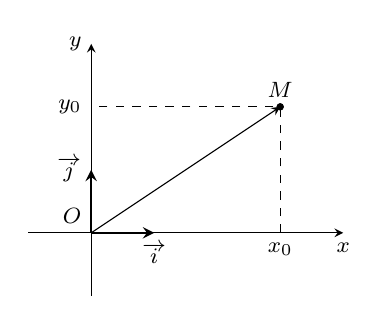
\begin{tikzpicture}[smooth,font=\footnotesize,scale=0.8,>=stealth]
		\draw[->] (-1,0)--(4,0) node [below]{$x$};
		\draw[->] (0,-1)--(0,3) node [left]{$y$};
		\draw[->,thick] (0,0)--(1,0) node [below]{$\overrightarrow{i}$};
		\draw[->,thick] (0,0)--(0,1) node [left]{$\overrightarrow{j}$};
		\draw (0,0) node[above left]{$O$};
		\draw[->] (0,0)--(3,2);
		\draw[dashed] (3,0)node [below]{$x_0$}--(3,2)node [above]{$M$}--(0,2)node [left]{$y_0$} ;
		\draw [fill=black] (3,2) circle (.05);
		%\node[below right] at (1.5,1.2){$\vec{u}$};
\end{tikzpicture}}
\subsubsection{Tọa độ của vectơ}
\vspace{-0.5cm}
\immini{\begin{itemize}
	\item [\iconMT] \indam{Định nghĩa:} Với mỗi vectơ $\vec{u}$ trên mặt phẳng $Oxy$, có duy nhất cặp số $(x_0;y_0)$ sao cho $\vec{u}=x_0\vec{i}+y_0\vec{j}$. Ta nói $\vec{u}$ có tọa độ là $(x_0;y_0)$ và viết $\vec{u}=(x_0;y_0)$ hoặc $\vec{u}(x_0;y_0)$.
	\item [\iconMT] \indam{Chú ý:}
	\begin{boxkn}
	\begin{itemize}
		\item Tọa độ hai vectơ đơn vị là $\vec{i}=(1;0)$, $\vec{j}=(0;1)$.
		\item $\overrightarrow{u}(x;y)=\overrightarrow{v}(x';y')\Leftrightarrow \heva{&x=x'\\ & y=y'}$.
	\end{itemize}
	\end{boxkn}
\end{itemize}}{\vspace{1cm}
		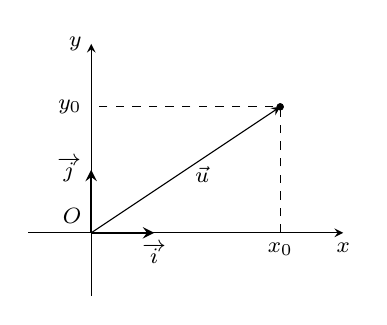
\begin{tikzpicture}[smooth,font=\footnotesize,scale=0.8,>=stealth]
		\draw[->] (-1,0)--(4,0) node [below]{$x$};
		\draw[->] (0,-1)--(0,3) node [left]{$y$};
		\draw[->,thick] (0,0)--(1,0) node [below]{$\overrightarrow{i}$};
		\draw[->,thick] (0,0)--(0,1) node [left]{$\overrightarrow{j}$};
		\draw (0,0) node[above left]{$O$};
		\draw[->] (0,0)--(3,2);
		\draw[dashed] (3,0)node [below]{$x_0$}--(3,2)--(0,2)node [left]{$y_0$} ;
		\draw [fill=black] (3,2) circle (.05);
		\node[below right] at (1.5,1.2){$\vec{u}$};
\end{tikzpicture}}

\subsubsection{Biểu thức tọa độ của các phép toán vectơ}
Cho hai vectơ $\overrightarrow{a}=\left( a_1;a_2 \right)$ và $\overrightarrow{b}=\left( b_1;b_2\right)$. Khi đó
\begin{tcolorbox}[colframe=cyan,colback=white,boxrule=0.2mm]
	\begin{listEX}[2]
		\item [\ding{172}] $\overrightarrow{a}+ \overrightarrow{b}=\left( a_1+ b_1;a_2+ b_2 \right)$ .
		\item [\ding{173}] $\overrightarrow{a}-\overrightarrow{b}=\left( a_1- b_1;a_2- b_2 \right)$ .
		\item [\ding{174}] $k\overrightarrow{a}=\left( ka_1;ka_2\right)$, với $k$ là một hằng số.
	\end{listEX}
\end{tcolorbox}
\subsubsection{Tọa độ điểm}
Cho ba điểm $A\left( x_A;y_A \right)$, $B\left( x_B;y_B\right)$ và $C\left( x_C;y_C\right)$. Khi đó
\begin{tcolorbox}[colframe=cyan,colback=white,boxrule=0.2mm]
	\begin{listEX}[1]
		\item [\ding{172}] $\overrightarrow{AB}=\left( x_B-x_A;y_B-y_A\right)$ 
		\item [\ding{173}] Khoảng cách giữa hai điểm $A$, $B$ là $AB=\sqrt{\left( x_B-x_A\right)^2+\left(y_B-y_A\right)^2}$.
		\item [\ding{174}] Trung điểm $I$ của $AB$:	$x_I=\dfrac{x_A+x_B}{2}$ và $y_I=\dfrac{y_A+y_B}{2}$
		\item [\ding{175}] $G$ là trọng tâm tam giác $ABC$: 
		$x_G=\dfrac{x_A+x_B+x_C}{3}$ và $y_G=\dfrac{y_A+y_B+y_C}{3}$.
		\item [\ding{176}] $ABC$ là ba đỉnh của tam giác $\Leftrightarrow $ $\overrightarrow{AB}$ không cùng phương với $\overrightarrow{AC}$
\end{listEX}
\end{tcolorbox}

\subsection{RÈN LUYỆN KĨ NĂNG GIẢI TOÁN}

\begin{dang}{Tìm tọa độ vec tơ}
	
\end{dang}

\begin{vd}
	Viết tọa độ của các vectơ sau
	\begin{tasks}(3)
		\task $\overrightarrow{a}=2\overrightarrow{i}+3\overrightarrow{j}$.
		\task $\overrightarrow{b}=\dfrac{1}{3}\overrightarrow{i}-5\overrightarrow{j}$.
		\task $\overrightarrow{c}=3\overrightarrow{i}$.
	\end{tasks}
	\loigiai{
	Ta nhắc lại lí thuyết: Vectơ $\vec{u} = x\vec{i} + y\vec{j}$ có tọa độ là $(x; y)$.
	\begin{enumerate}
		\item[a)] Ta có $\vec{a} = 2\vec{i} + 3\vec{j} \Rightarrow \vec{a} = (2; 3)$.
		\item[b)] Ta có $\vec{b} = \dfrac{1}{3}\vec{i} - 5\vec{j} \Rightarrow \vec{b} = \left(\dfrac{1}{3}; -5\right)$.
		\item[c)] Ta có $\vec{c} = 3\vec{i} = 3\vec{i} + 0\vec{j} \Rightarrow \vec{c} = (3; 0)$.
	\end{enumerate}
}
\end{vd}\dongcham{3}

\begin{vd}
	Cho $\overrightarrow{a}=(1;-2)$, $\overrightarrow{b}=(0;3)$. Tìm toạ độ của các vectơ sau
	\begin{tasks}(1)
		\task $\overrightarrow{x}=\overrightarrow{a}+\overrightarrow{b}$;\quad $\overrightarrow{y}=\overrightarrow{a}-\overrightarrow{b}$;\quad $\overrightarrow{z}=2\overrightarrow{a}-3\overrightarrow{b}$.
		\task $\overrightarrow{u}=3\overrightarrow{a}-2\overrightarrow{b}$;\quad $\overrightarrow{v}=2\overrightarrow{a}+\overrightarrow{b}$;\quad $\overrightarrow{w}=4\overrightarrow{a}-\dfrac{1}{2}\overrightarrow{b}$.
	\end{tasks}
	\loigiai{
	\begin{enumerate}
		\item[a)] Ta thực hiện phép toán tọa độ:
		\begin{itemize}
			\item $\vec{x} = \vec{a} + \vec{b} = (1 + 0; -2 + 3) = (1; 1)$.
			\item $\vec{y} = \vec{a} - \vec{b} = (1 - 0; -2 - 3) = (1; -5)$.
			\item $\vec{z} = 2\vec{a} - 3\vec{b} = 2(1; -2) - 3(0; 3) = (2; -4) - (0; 9) = (2 - 0; -4 - 9) = (2; -13)$.
		\end{itemize}
		\item[b)] Tương tự, ta có:
		\begin{itemize}
			\item $\vec{u} = 3\vec{a} - 2\vec{b} = 3(1; -2) - 2(0; 3) = (3; -6) - (0; 6) = (3 - 0; -6 - 6) = (3; -12)$.
			\item $\vec{v} = 2\vec{a} + \vec{b} = 2(1; -2) + (0; 3) = (2; -4) + (0; 3) = (2 + 0; -4 + 3) = (2; -1)$.
			\item $\vec{w} = 4\vec{a} - \dfrac{1}{2}\vec{b} = 4(1; -2) - \dfrac{1}{2}(0; 3) = (4; -8) - \left(0; \dfrac{3}{2}\right) = \left(4 - 0; -8 - \dfrac{3}{2}\right) = \left(4; -\dfrac{19}{2}\right)$.
		\end{itemize}
	\end{enumerate}
}
\end{vd}\dongcham{4}

\begin{vd}
	Cho $\overrightarrow{a}=(2;1)$, $\overrightarrow{b}=(3;4)$, $\overrightarrow{c}=(7;2)$.
	\begin{tasks}(1)
		\task Tìm tọa độ của vectơ $\overrightarrow{u}=2\overrightarrow{a}-3\,\overrightarrow{b}$.
		\task Tìm tọa độ của vectơ $\overrightarrow{x}$ sao cho $\overrightarrow{x}+\overrightarrow{a}=\overrightarrow{b}-\overrightarrow{c}$.
	\end{tasks}
	\loigiai{
	\begin{enumerate}
		\item[a)] Ta có:
		$$ \vec{u} = 2\vec{a} - 3\vec{b} = 2(2; 1) - 3(3; 4) = (4; 2) - (9; 12) = (4 - 9; 2 - 12) = (-5; -10). $$
		\item[b)] Từ phương trình vectơ $\vec{x} + \vec{a} = \vec{b} - \vec{c}$, ta chuyển vế để tìm $\vec{x}$:
		$$ \vec{x} = \vec{b} - \vec{c} - \vec{a} $$
		Thay tọa độ các vectơ vào, ta được:
		$$ \vec{x} = (3; 4) - (7; 2) - (2; 1) = (3 - 7 - 2; 4 - 2 - 1) = (-6; 1). $$
		Vậy $\vec{x} = (-6; 1)$.
	\end{enumerate}
}
\end{vd}\dongcham{5}

\begin{vd}
	Cho $\overrightarrow{a}=(-2;0)$, $\overrightarrow{b}=(3;4)$, $\overrightarrow{c}=(7;2)$. Tính tọa độ vectơ
	\begin{tasks}(2)
		\task  $\overrightarrow{u}=2\overrightarrow{a}-4\overrightarrow{b}+\overrightarrow{c}$.
		\task $\overrightarrow{v}=-\overrightarrow{a}+\dfrac{1}{3}\cdot\overrightarrow{b}-\dfrac{1}{2}\cdot\overrightarrow{c}$.
	\end{tasks}
	\loigiai{
	\begin{enumerate}
		\item[a)] Ta thay tọa độ các vectơ vào biểu thức:
		$$ \vec{u} = 2(-2; 0) - 4(3; 4) + (7; 2) $$
		$$ \vec{u} = (-4; 0) - (12; 16) + (7; 2) $$
		$$ \vec{u} = (-4 - 12 + 7; 0 - 16 + 2) = (-9; -14). $$
		\item[b)] Tương tự, ta tính tọa độ vectơ $\vec{v}$:
		$$ \vec{v} = -(-2; 0) + \dfrac{1}{3}(3; 4) - \dfrac{1}{2}(7; 2) $$
		$$ \vec{v} = (2; 0) + \left(1; \dfrac{4}{3}\right) - \left(\dfrac{7}{2}; 1\right) $$
		Gộp các hoành độ và tung độ lại với nhau:
		$$ \vec{v} = \left(2 + 1 - \dfrac{7}{2}; 0 + \dfrac{4}{3} - 1\right) = \left(3 - \dfrac{7}{2}; \dfrac{1}{3}\right) = \left(-\dfrac{1}{2}; \dfrac{1}{3}\right). $$
	\end{enumerate}
}
\end{vd}\dongcham{5}
\begin{dang}{Hai véc tơ cùng phương}
	 Cho hai vectơ $\overrightarrow{a}=\left( a_1;a_2 \right)$ và $\overrightarrow{b}=\left( b_1;b_2\right)$.  
	 \begin{itemize}
	 	\item [\iconMT] Điều kiện cần và đủ để $\overrightarrow{a}$ và $\overrightarrow{b} \ne \overrightarrow{0}$ cùng phương là $\exists k \in \mathbb{R} \colon \overrightarrow{a}=k\overrightarrow{b} \Leftrightarrow \heva{&a_1=kb_1\\&a_2=kb_2}$.
	 	\item [\iconMT] Nếu $b_1$ và $b_2$ khác $0$ thì $\overrightarrow{a}$ và $\overrightarrow{b} \ne \overrightarrow{0}$ cùng phương khi  $\dfrac{a_1}{b_1}=\dfrac{a_2}{b_2}$.
	 
	 \end{itemize}
\end{dang}

\begin{vd}
	Cặp vectơ nào sau đây cùng phương? cùng hướng? ngược hướng?
	\begin{tasks}(2)
		\task $\vec{a}=(1;2)$ và $\vec{b}=(2;4)$.
		\task $\vec{a}=(-3;2)$ và $\vec{b}=(1;2)$.
		\task $\vec{a}=(3;0)$ và $\vec{b}=(2;0)$.
		\task $\vec{a}=(4;-2)$ và $\vec{b}=(-2;1)$.
		\task $\vec{a}=(0;5)$ và $\vec{b}=(4;0)$.
		\task $\vec{a}=(0;2)$ và $\vec{b}=(0;-3)$.
	\end{tasks}
		\loigiai{
		Hai vectơ $\vec{u}$ và $\vec{v}$ (khác $\vec{0}$) cùng phương khi và chỉ khi tồn tại số thực $k \neq 0$ sao cho $\vec{u} = k\vec{v}$.
		\begin{itemize}
			\item Nếu $k > 0$ thì hai vectơ cùng hướng.
			\item Nếu $k < 0$ thì hai vectơ ngược hướng.
		\end{itemize}
		\begin{enumerate}
			\item[a)] Ta có $\vec{b} = (2; 4) = 2(1; 2) = 2\vec{a}$. Vì $k = 2 > 0$ nên hai vectơ $\vec{a}$ và $\vec{b}$ cùng phương và cùng hướng.
			\item[b)] Ta thấy $\dfrac{-3}{1} \neq \dfrac{2}{2}$ nên hai vectơ $\vec{a}$ và $\vec{b}$ không cùng phương.
			\item[c)] Ta có $\vec{a} = (3; 0) = \dfrac{3}{2}(2; 0) = \dfrac{3}{2}\vec{b}$. Vì $k = \dfrac{3}{2} > 0$ nên hai vectơ $\vec{a}$ và $\vec{b}$ cùng phương và cùng hướng.
			\item[d)] Ta có $\vec{a} = (4; -2) = -2(-2; 1) = -2\vec{b}$. Vì $k = -2 < 0$ nên hai vectơ $\vec{a}$ và $\vec{b}$ cùng phương và ngược hướng.
			\item[e)] Ta thấy $0 \cdot 0 - 5 \cdot 4 = -20 \neq 0$ (hoặc không tồn tại số $k$ nào thỏa mãn) nên hai vectơ $\vec{a}$ và $\vec{b}$ không cùng phương.
			\item[f)] Ta có $\vec{b} = (0; -3) = -\dfrac{3}{2}(0; 2) = -\dfrac{3}{2}\vec{a}$. Vì $k = -\dfrac{3}{2} < 0$ nên hai vectơ $\vec{a}$ và $\vec{b}$ cùng phương và ngược hướng.
		\end{enumerate}
	}
\end{vd}\dongcham{13}

\begin{vd}
	Cho $\overrightarrow{a}=(2;1)$, $\overrightarrow{b}=(m^2-m;3)$. Tìm $m$ để hai véc tơ $\overrightarrow{a}$ và $\overrightarrow{b}$ cùng phương.
		\loigiai{
		Hai vectơ $\vec{a} = (2; 1)$ và $\vec{b} = (m^2 - m; 3)$ cùng phương khi và chỉ khi tọa độ của chúng tương lệ (do tọa độ của $\vec{a}$ đều khác $0$). Ta có phương trình:
		$$ \dfrac{m^2 - m}{2} = \dfrac{3}{1} $$
		$$ \Leftrightarrow m^2 - m = 6 $$
		$$ \Leftrightarrow m^2 - m - 6 = 0 $$
		$$ \Leftrightarrow \hoac{m &= 3 \\ m &= -2} $$
		Vậy với $m = 3$ hoặc $m = -2$ thì hai vectơ $\vec{a}$ và $\vec{b}$ cùng phương.
	}
\end{vd}\dongcham{4}

\begin{vd}%[0H1G4-5]%
	Trong mặt phẳng tọa độ $Oxy$, cho $\vec{a}=(m;2)$, $\vec{b}=(1-m;m+4)$ (với $m$ là tham số). Tìm $m$ sao cho $2\vec{a}-3\vec{b}$ cùng phương với $\vec{c}=(4;-2)$.
	\loigiai{
		Ta có $\vec{d}=2\vec{a}-3\vec{b}=(5m-3;-3m-8)$. Hai véc-tơ $\vec{d}$, $\vec{c}$ cùng phương khi và chỉ khi $$(5m-3)\cdot (-2)=(-3m-8)\cdot 4\Leftrightarrow m=-19.$$
	}
\end{vd}\dongcham{8}
\begin{dang}{Phân tích vectơ theo hai vectơ không cùng phương}
	Giả sử cần phân tích $\vec{u}=(u_1;u_2)$ theo hai vectơ không cùng phương $\vec{a}=(a_1;a_2)$ và $\vec{b}=(b_1;b_2)$. Ta thực hiện như sau:
	\begin{itemize}
		\item [$\bullet$] Giả sử $\vec{u} =m \cdot \vec{a} + n \cdot \vec{b}$ với $m,n \in \mathbb{R}$.
		\item [$\bullet$] Dùng điều kiện vectơ bằng nhau, ta được hệ
		$\heva{&u_1=m\cdot a_1 + n\cdot b_1\\&u_2=m\cdot a_2 + n\cdot b_2}.$
		\item [$\bullet$] Giải hệ trên tìm $m$ và $n$. Kết luận $\vec{u} =m \cdot \vec{a} + n \cdot \vec{b}$ với $m$, $n$ vừa tìm được.
	\end{itemize}
	
\end{dang}
\begin{vd}
	Phân tích vectơ $\overrightarrow{u}$ theo hai vectơ $\overrightarrow{a}$ và $\overrightarrow{b}$, biết
	\begin{tasks}(2)
		\task $\overrightarrow{u}=(-4;7)$, $\overrightarrow{a}=(2;-1)$, $\overrightarrow{b}=(-3;4)$.
		\task $\overrightarrow{u}=(-1;3)$, $\overrightarrow{a}=(1;1)$, $\overrightarrow{b}=(2;3)$.
		\task $\overrightarrow{u}=(-1;3)$, $\overrightarrow{a}=(2;1)$, $\overrightarrow{b}=(3;2)$.
		\task $\overrightarrow{u}=2\overrightarrow{i}-3\overrightarrow{j}$, $\overrightarrow{a}=(1;1)$, $\overrightarrow{b}=(2;3)$.
	\end{tasks}
	\loigiai{
	Giả sử $\vec{u} = x\vec{a} + y\vec{b}$ ($x, y \in \mathbb{R}$). Ta thiết lập hệ phương trình tọa độ tương ứng:
	\begin{enumerate}
		\item[a)] Ta có hệ phương trình:
		$$ \heva{2x - 3y &= -4 \\ -x + 4y &= 7} \Leftrightarrow \heva{2x - 3y &= -4 \\ -2x + 8y &= 14} \Leftrightarrow \heva{5y &= 10 \\ x &= 4y - 7} \Leftrightarrow \heva{y &= 2 \\ x &= 1} $$
		Vậy $\vec{u} = \vec{a} + 2\vec{b}$.
		
		\item[b)] Ta có hệ phương trình:
		$$ \heva{x + 2y &= -1 \\ x + 3y &= 3} \Leftrightarrow \heva{y &= 4 \\ x &= -1 - 2y} \Leftrightarrow \heva{y &= 4 \\ x &= -9} $$
		Vậy $\vec{u} = -9\vec{a} + 4\vec{b}$.
		
		\item[c)] Ta có hệ phương trình:
		$$ \heva{2x + 3y &= -1 \\ x + 2y &= 3} \Leftrightarrow \heva{x &= 3 - 2y \\ 2(3 - 2y) + 3y &= -1} \Leftrightarrow \heva{x &= 3 - 2y \\ -y &= -7} \Leftrightarrow \heva{x &= -11 \\ y &= 7} $$
		Vậy $\vec{u} = -11\vec{a} + 7\vec{b}$.
		
		\item[d)] Ta có $\vec{u} = 2\vec{i} - 3\vec{j} \Rightarrow \vec{u} = (2; -3)$. Ta có hệ phương trình:
		$$ \heva{x + 2y &= 2 \\ x + 3y &= -3} \Leftrightarrow \heva{y &= -5 \\ x &= 2 - 2y} \Leftrightarrow \heva{y &= -5 \\ x &= 12} $$
		Vậy $\vec{u} = 12\vec{a} - 5\vec{b}$.
	\end{enumerate}
}
\end{vd}\dongcham{18}


\begin{dang}{Tìm tọa độ điểm}
	Các bài toán thường gặp
	\begin{listEX}[1]
		\item [\ding{172}] Tìm điểm $I$ là trung điểm của đoạn thẳng cho trước.
		\item [\ding{173}] Tìm điểm $G$ là trọng tâm của tam giác cho trước.
		\item [\ding{174}] Tìm điểm $M$ thỏa mãn một đẳng thức vectơ.
		\item [\ding{175}] Tìm điểm $M$ trên $Ox$ hoặc $Oy$ cùng với hai điểm cho trước thẳng hàng.
		\item [\ding{176}] Tìm điểm $D$ sao cho tứ giác $ABCD$ là hình bình hành.
	\end{listEX}
\end{dang}
\begin{vd}
	Trên mặt phẳng $Oxy$, cho 2 điểm $A\left( -2;-2 \right)$ và $B\left( 5;-4 \right)$.
	\begin{tasks}
		\task Tìm tọa độ trọng tâm của tam giác $OAB$.
		\task 	Tìm tọa độ điểm $C$ sao cho tam giác $ABC$ có trọng tâm là điểm $G\left( 2;0 \right)$.
	\end{tasks}
	\loigiai{
	Ta có gốc tọa độ $O(0; 0)$.
	\begin{enumerate}
		\item[a)] Gọi $G_{1}$ là trọng tâm tam giác $OAB$. Áp dụng công thức tọa độ trọng tâm:
		$$ \heva{x_{G_1} &= \dfrac{x_O + x_A + x_B}{3} = \dfrac{0 - 2 + 5}{3} = 1 \\ y_{G_1} &= \dfrac{y_O + y_A + y_B}{3} = \dfrac{0 - 2 - 4}{3} = -2} $$
		Vậy trọng tâm của tam giác $OAB$ là điểm $(1; -2)$.
		
		\item[b)] Gọi $C(x_C; y_C)$. Vì $G(2; 0)$ là trọng tâm tam giác $ABC$ nên ta có:
		$$ \heva{x_G &= \dfrac{x_A + x_B + x_C}{3} \\ y_G &= \dfrac{y_A + y_B + y_C}{3}} \Leftrightarrow \heva{3x_G &= x_A + x_B + x_C \\ 3y_G &= y_A + y_B + y_C} \Leftrightarrow \heva{x_C &= 3x_G - x_A - x_B \\ y_C &= 3y_G - y_A - y_B} $$
		Thay số vào ta được:
		$$ \heva{x_C &= 3(2) - (-2) - 5 = 6 + 2 - 5 = 3 \\ y_C &= 3(0) - (-2) - (-4) = 0 + 2 + 4 = 6} $$
		Vậy tọa độ điểm $C$ cần tìm là $C(3; 6)$.
	\end{enumerate}
}
\end{vd}\dongcham{6}

\begin{vd}
	Trên mặt phẳng $Oxy$, cho ba điểm $A(-3;4)$, $B(1;1)$, $C(2;-5)$.
	\begin{tasks}(1)
		\task Chứng minh ba điểm $A$, $B$, $C$ không thẳng hàng.
		\task Gọi $M$, $N$, $P$ lần lượt là trung điểm của $AB$, $BC$, $CA$. Tìm tọa độ $M$, $N$, $P$.
		\task Tìm tọa độ điểm $D$ sao cho $ABCD$ là hình bình hành.
		\task Tìm tọa độ điểm $E$ trên trục tung sao cho $\overrightarrow{AE}$ và $\overrightarrow{BC}$ cùng phương.
	\end{tasks}
	\loigiai{
	\begin{enumerate}
		\item[a)] Ta có $\overrightarrow{AB} = (1 - (-3); 1 - 4) = (4; -3)$ và $\overrightarrow{AC} = (2 - (-3); -5 - 4) = (5; -9)$.\\
		Vì $\dfrac{4}{5} \neq \dfrac{-3}{-9}$ nên hai vectơ $\overrightarrow{AB}$ và $\overrightarrow{AC}$ không cùng phương.\\
		Suy ra ba điểm $A, B, C$ không thẳng hàng.
		
		\item[b)] Áp dụng công thức tọa độ trung điểm:
		\begin{itemize}
			\item $M$ là trung điểm $AB$: $M\left(\dfrac{-3 + 1}{2}; \dfrac{4 + 1}{2}\right) \Rightarrow M\left(-1; \dfrac{5}{2}\right)$.
			\item $N$ là trung điểm $BC$: $N\left(\dfrac{1 + 2}{2}; \dfrac{1 - 5}{2}\right) \Rightarrow N\left(\dfrac{3}{2}; -2\right)$.
			\item $P$ là trung điểm $CA$: $P\left(\dfrac{2 - 3}{2}; \dfrac{-5 + 4}{2}\right) \Rightarrow P\left(-\dfrac{1}{2}; -\dfrac{1}{2}\right)$.
		\end{itemize}
		
		\item[c)] Gọi $D(x; y)$. Tứ giác $ABCD$ là hình bình hành khi và chỉ khi $\overrightarrow{AB} = \overrightarrow{DC}$.\\
		Ta có $\overrightarrow{AB} = (4; -3)$ và $\overrightarrow{DC} = (2 - x; -5 - y)$.\\
		Suy ra:
		$$ \heva{2 - x &= 4 \\ -5 - y &= -3} \Leftrightarrow \heva{x &= -2 \\ y &= -2} $$
		Vậy $D(-2; -2)$.
		
		\item[d)] Vì $E$ nằm trên trục tung nên gọi tọa độ của $E$ là $E(0; y)$.\\
		Ta có $\overrightarrow{AE} = (0 - (-3); y - 4) = (3; y - 4)$.\\
		Mặt khác $\overrightarrow{BC} = (2 - 1; -5 - 1) = (1; -6)$.\\
		Hai vectơ $\overrightarrow{AE}$ và $\overrightarrow{BC}$ cùng phương khi tọa độ của chúng tương lệ:
		$$ \dfrac{3}{1} = \dfrac{y - 4}{-6} \Leftrightarrow y - 4 = -18 \Leftrightarrow y = -14. $$
		Vậy điểm cần tìm là $E(0; -14)$.
	\end{enumerate}
}
\end{vd}\dongcham{15}

\begin{vd}
	Cho tam giác $ABC$. Biết các điểm $M(1;1)$, $N(2;3)$, $P(0;4)$ lần lượt là trung điểm các cạnh $AB$, $BC$, $CA$.
	\begin{tasks}(1)
		\task Tìm tọa độ các đỉnh $A$, $B$, $C$.
		\task Tìm tọa độ trọng tâm $G$ của tam giác $ABC$.
	\end{tasks}
	\loigiai{
	\begin{enumerate}
		\item[a)] Vì $M, N, P$ lần lượt là trung điểm của $AB, BC, CA$ nên tứ giác $AMPN$, $BMNP$ và $CMPN$ là các hình bình hành.\\
		Ta có $\overrightarrow{NM} = (1 - 2; 1 - 3) = (-1; -2)$.\\
		Vì $AMPN$ là hình bình hành nên $\overrightarrow{PA} = \overrightarrow{NM} \Leftrightarrow \heva{x_A - 0 &= -1 \\ y_A - 4 &= -2} \Leftrightarrow \heva{x_A &= -1 \\ y_A &= 2} \Rightarrow A(-1; 2)$.\\
		Ta có $\overrightarrow{PN} = (2 - 0; 3 - 4) = (2; -1)$.\\
		Vì $MNPB$ là hình bình hành nên $\overrightarrow{MB} = \overrightarrow{PN} \Leftrightarrow \heva{x_B - 1 &= 2 \\ y_B - 1 &= -1} \Leftrightarrow \heva{x_B &= 3 \\ y_B &= 0} \Rightarrow B(3; 0)$.\\
		Ta có $\overrightarrow{MP} = (0 - 1; 4 - 1) = (-1; 3)$.\\
		Vì $NPCM$ là hình bình hành nên $\overrightarrow{NC} = \overrightarrow{MP} \Leftrightarrow \heva{x_C - 2 &= -1 \\ y_C - 3 &= 3} \Leftrightarrow \heva{x_C &= 1 \\ y_C &= 6} \Rightarrow C(1; 6)$.\\
		Vậy $A(-1; 2)$, $B(3; 0)$, $C(1; 6)$.
		
		\item[b)] Trọng tâm $G$ của tam giác $ABC$ có tọa độ là:
		$$ \heva{x_G &= \dfrac{x_A + x_B + x_C}{3} = \dfrac{-1 + 3 + 1}{3} = 1 \\ y_G &= \dfrac{y_A + y_B + y_C}{3} = \dfrac{2 + 0 + 6}{3} = \dfrac{8}{3}} $$
		Vậy $G\left(1; \dfrac{8}{3}\right)$.
	\end{enumerate}
}
\end{vd}\dongcham{12}

\begin{vd}
	Cho ba điểm $A(-1; 2)$, $B (3; -4)$, $C(5; 0)$. Tìm tọa độ điểm $D$ nếu biết
	\begin{tasks}(1)
		\task $\overrightarrow{AD}-2\overrightarrow{BD}+3\overrightarrow{CD}=\overrightarrow{0}$.
		\task $\overrightarrow{AD}-2\overrightarrow{AB}=2\overrightarrow{BD}+\overrightarrow{BC}$.
		\task tứ giác $ABCD$ hình bình hành.
		\task tứ giác $ABCD$ hình thang có hai đáy là $BC$, $AD$ với $BC = 2AD$.
	\end{tasks}
	\loigiai{
	Gọi $D(x; y)$.
	\begin{enumerate}
		\item[a)] Ta có $\overrightarrow{AD} = (x + 1; y - 2)$, $\overrightarrow{BD} = (x - 3; y + 4)$, $\overrightarrow{CD} = (x - 5; y)$.\\
		Từ giả thiết $\overrightarrow{AD} - 2\overrightarrow{BD} + 3\overrightarrow{CD} = \vec{0}$, ta có hệ phương trình:
		$$ \heva{(x + 1) - 2(x - 3) + 3(x - 5) &= 0 \\ (y - 2) - 2(y + 4) + 3y &= 0} \Leftrightarrow \heva{x + 1 - 2x + 6 + 3x - 15 &= 0 \\ y - 2 - 2y - 8 + 3y &= 0} \Leftrightarrow \heva{2x - 8 &= 0 \\ 2y - 10 &= 0} \Leftrightarrow \heva{x &= 4 \\ y &= 5} $$
		Vậy $D(4; 5)$.
		
		\item[b)] Ta có phương trình: $\overrightarrow{AD} - 2\overrightarrow{BD} = 2\overrightarrow{AB} + \overrightarrow{BC}$.\\
		Tính tọa độ các vectơ: $\overrightarrow{AB} = (4; -6) \Rightarrow 2\overrightarrow{AB} = (8; -12)$; $\overrightarrow{BC} = (2; 4)$.\\
		Vế phải: $2\overrightarrow{AB} + \overrightarrow{BC} = (8 + 2; -12 + 4) = (10; -8)$.\\
		Vế trái: $\overrightarrow{AD} - 2\overrightarrow{BD} = (x + 1 - 2(x - 3); y - 2 - 2(y + 4)) = (-x + 7; -y - 10)$.\\
		Đồng nhất hai vế ta được:
		$$ \heva{-x + 7 &= 10 \\ -y - 10 &= -8} \Leftrightarrow \heva{x &= -3 \\ y &= -2} $$
		Vậy $D(-3; -2)$.
		
		\item[c)] Tứ giác $ABCD$ là hình bình hành khi và chỉ khi $\overrightarrow{AB} = \overrightarrow{DC}$.\\
		Ta có $\overrightarrow{AB} = (4; -6)$ và $\overrightarrow{DC} = (5 - x; 0 - y) = (5 - x; -y)$.\\
		Suy ra: $ \heva{5 - x &= 4 \\ -y &= -6} \Leftrightarrow \heva{x &= 1 \\ y &= 6} $. Vậy $D(1; 6)$.
		
		\item[d)] Tứ giác $ABCD$ là hình thang có hai đáy là $BC$ và $AD$ (theo đúng thứ tự vòng quanh đỉnh của đa giác) nên hai vectơ $\overrightarrow{BC}$ và $\overrightarrow{AD}$ cùng hướng. Mặt khác $BC = 2AD$ nên ta có $\overrightarrow{BC} = 2\overrightarrow{AD}$.\\
		Ta có $\overrightarrow{BC} = (2; 4)$ và $\overrightarrow{AD} = (x + 1; y - 2)$. Suy ra:
		$$ \heva{2(x + 1) &= 2 \\ 2(y - 2) &= 4} \Leftrightarrow \heva{x + 1 &= 1 \\ y - 2 &= 2} \Leftrightarrow \heva{x &= 0 \\ y &= 4} $$
		Vậy $D(0; 4)$.
	\end{enumerate}
}
\end{vd}\dongcham{18}

\begin{vd}
	Cho hai điểm $I(1; -3)$, $J(-2; 4)$ chia đọan $AB$ thành ba đọan bằng nhau $AI = IJ = JB$.
	\begin{tasks}(1)
		\task Tìm tọa độ của $A$, $B$.
		\task Tìm tọa độ của điểm $I'$ đối xứng với $I$ qua $B$.
		\task Tìm tọa độ của $C$, $D$ biết $ABCD$ hình bình hành tâm $K(5, -6)$.
	\end{tasks}
	\loigiai{
	Ta có $\overrightarrow{IJ} = (-2 - 1; 4 - (-3)) = (-3; 7)$.
	\begin{enumerate}
		\item[a)] Vì $AI = IJ$ và $I$ nằm giữa $A, J$ nên $\overrightarrow{AI} = \overrightarrow{IJ} \Leftrightarrow \heva{1 - x_A &= -3 \\ -3 - y_A &= 7} \Leftrightarrow \heva{x_A &= 4 \\ y_A &= -10} \Rightarrow A(4; -10)$.\\
		Vì $IJ = JB$ và $J$ nằm giữa $I, B$ nên $\overrightarrow{JB} = \overrightarrow{IJ} \Leftrightarrow \heva{x_B - (-2) &= -3 \\ y_B - 4 &= 7} \Leftrightarrow \heva{x_B &= -5 \\ y_B &= 11} \Rightarrow B(-5; 11)$.
		
		\item[b)] Vì $I'$ đối xứng với $I$ qua $B$ nên $B$ là trung điểm của đoạn thẳng $II'$. Ta có:
		$$ \heva{x_{I'} &= 2x_B - x_I = 2(-5) - 1 = -11 \\ y_{I'} &= 2y_B - y_I = 2(11) - (-3) = 25} $$
		Vậy $I'(-11; 25)$.
		
		\item[c)] Vì $ABCD$ là hình bình hành tâm $K(5; -6)$ nên $K$ là trung điểm của các đường chéo $AC$ và $BD$.
		$$ \heva{x_C &= 2x_K - x_A = 2(5) - 4 = 6 \\ y_C &= 2y_K - y_A = 2(-6) - (-10) = -2} \Rightarrow C(6; -2). $$
		$$ \heva{x_D &= 2x_K - x_B = 2(5) - (-5) = 15 \\ y_D &= 2y_K - y_B = 2(-6) - 11 = -23} \Rightarrow D(15; -23). $$
		Vậy $C(6; -2)$ và $D(15; -23)$.
	\end{enumerate}
}
\end{vd}\dongcham{13}

\begin{vd}
	Cho ba điểm $A\left( 1;1 \right)$, $B\left( 3;2 \right)$ và $C\left( m+4;2m+1 \right)$ . Tìm $m$ để ba điểm $A$, $B$, $C$ thẳng hàng.
		\loigiai{
		Ta có $\overrightarrow{AB} = (2; 1)$ và $\overrightarrow{AC} = (m + 3; 2m)$.\\
		Ba điểm $A, B, C$ thẳng hàng khi và chỉ khi hai vectơ $\overrightarrow{AB}$ và $\overrightarrow{AC}$ cùng phương. Vì tọa độ của $\overrightarrow{AB}$ đều khác $0$ nên ta có tỉ lệ:
		$$ \dfrac{m + 3}{2} = \dfrac{2m}{1} \Leftrightarrow m + 3 = 4m \Leftrightarrow 3m = 3 \Leftrightarrow m = 1. $$
		Vậy $m = 1$ là giá trị cần tìm.
	}
\end{vd}\dongcham{10}

\begin{vd}
	Cho hai điểm $A\left( 3;4 \right),B\left( 2;5 \right)$ . Tìm $x$ để điểm $C\left( -7;x \right)$ thuộc đường thẳng $AB$.
		\loigiai{
		Điểm $C$ thuộc đường thẳng $AB$ khi và chỉ khi ba điểm $A, B, C$ thẳng hàng, tức là hai vectơ $\overrightarrow{AB}$ và $\overrightarrow{AC}$ cùng phương.\\
		Ta có $\overrightarrow{AB} = (-1; 1)$ và $\overrightarrow{AC} = (-10; x - 4)$.\\
		Để hai vectơ cùng phương, ta có điều kiện:
		$$ \dfrac{-10}{-1} = \dfrac{x - 4}{1} \Leftrightarrow 10 = x - 4 \Leftrightarrow x = 14. $$
		Vậy $x = 14$ là giá trị cần tìm.
	}
\end{vd}\dongcham{10}

\begin{dang}{Tính độ dài đoạn thẳng} 
	Chú ý các công thức sau:
	\begin{itemize}
		\item [$\bullet$] $\overrightarrow{AB}=\left( x_B-x_A;y_B-y_A\right)$ 
		\item [$\bullet$] Khoảng cách giữa hai điểm $A$, $B$ là $AB=\sqrt{\left( x_B-x_A\right)^2+\left(y_B-y_A\right)^2}$.
	\end{itemize}
\end{dang}

\begin{vd}
	Trong mặt phẳng $Oxy$, cho tam giác $ABC$ với $A(1;4)$, $B(2;2)$, $C(8;5)$.
	\begin{tasks}(1)
		\task Tính độ dài các cạnh của tam giác $ABC$. Chứng tỏ tam giác $ABC$ vuông tại $B$.
		\task Tính chu vi và diện tích tam giác $ABC$ (kết quả làm tròn đến 2 chữ số thập phân).
	\end{tasks}
	\loigiai{
	\begin{enumerate}
		\item[a)] Áp dụng công thức tính khoảng cách giữa hai điểm:
		\begin{itemize}
			\item $AB = \sqrt{(2 - 1)^2 + (2 - 4)^2} = \sqrt{1^2 + (-2)^2} = \sqrt{5}$.
			\item $BC = \sqrt{(8 - 2)^2 + (5 - 2)^2} = \sqrt{6^2 + 3^2} = \sqrt{36 + 9} = \sqrt{45} = 3\sqrt{5}$.
			\item $AC = \sqrt{(8 - 1)^2 + (5 - 4)^2} = \sqrt{7^2 + 1^2} = \sqrt{49 + 1} = \sqrt{50} = 5\sqrt{2}$.
		\end{itemize}
		Ta xét các bình phương độ dài: $AB^2 = 5$, $BC^2 = 45$, $AC^2 = 50$.\\
		Nhận thấy $AB^2 + BC^2 = 5 + 45 = 50 = AC^2$.\\
		Theo định lý Pythagore đảo, tam giác $ABC$ vuông tại $B$.
		
		\item[b)] Chu vi tam giác $ABC$ là:
		$$ P = AB + BC + AC = \sqrt{5} + 3\sqrt{5} + 5\sqrt{2} = 4\sqrt{5} + 5\sqrt{2} \approx 16{,}02. $$
		Vì tam giác $ABC$ vuông tại $B$ nên diện tích tam giác là:
		$$ S = \dfrac{1}{2} AB \cdot BC = \dfrac{1}{2} \cdot \sqrt{5} \cdot 3\sqrt{5} = \dfrac{15}{2} = 7{,}5. $$
	\end{enumerate}
}
\end{vd}\dongcham{12}

\begin{vd}
	Trong mặt phẳng $Oxy$, cho $A(-2;2)$, $B\left(\frac{5}{2};2+\frac{3\sqrt{3}}{2} \right)$, $C\left(\frac{5}{2};2-\frac{3\sqrt{3}}{2} \right)$
	\begin{tasks}(1)
		\task Tính độ dài các cạnh của tam giác $ABC$. Chứng tỏ tam giác $ABC$ đều.
		\task Tính diện tích tam giác $ABC$ (kết quả làm tròn đến 2 chữ số thập phân).
	\end{tasks}
	\loigiai{
	\begin{enumerate}
		\item[a)] Áp dụng công thức tính khoảng cách:
		\begin{itemize}
			\item $AB = \sqrt{\left(\dfrac{5}{2} - (-2)\right)^2 + \left(2 + \dfrac{3\sqrt{3}}{2} - 2\right)^2} = \sqrt{\left(\dfrac{9}{2}\right)^2 + \left(\dfrac{3\sqrt{3}}{2}\right)^2} = \sqrt{\dfrac{81}{4} + \dfrac{27}{4}} = \sqrt{\dfrac{108}{4}} = \sqrt{27} = 3\sqrt{3}$.
			\item $AC = \sqrt{\left(\dfrac{5}{2} - (-2)\right)^2 + \left(2 - \dfrac{3\sqrt{3}}{2} - 2\right)^2} = \sqrt{\left(\dfrac{9}{2}\right)^2 + \left(-\dfrac{3\sqrt{3}}{2}\right)^2} = \sqrt{\dfrac{81}{4} + \dfrac{27}{4}} = \sqrt{\dfrac{108}{4}} = \sqrt{27} = 3\sqrt{3}$.
			\item $BC = \sqrt{\left(\dfrac{5}{2} - \dfrac{5}{2}\right)^2 + \left(2 - \dfrac{3\sqrt{3}}{2} - \left(2 + \dfrac{3\sqrt{3}}{2}\right)\right)^2} = \sqrt{0^2 + (-3\sqrt{3})^2} = \sqrt{27} = 3\sqrt{3}$.
		\end{itemize}
		Vì $AB = BC = AC = 3\sqrt{3}$ nên tam giác $ABC$ là tam giác đều.
		
		\item[b)] Diện tích tam giác đều cạnh $a$ được tính theo công thức $S = \dfrac{a^2\sqrt{3}}{4}$.\\
		Với $a = 3\sqrt{3}$, ta có:
		$$ S = \dfrac{(3\sqrt{3})^2\sqrt{3}}{4} = \dfrac{27\sqrt{3}}{4} \approx 11{,}69. $$
	\end{enumerate}
}
\end{vd}\dongcham{15}

\begin{vd}
	Trong mặt phẳng $Oxy$, cho điểm $A(2;1)$ và $\vec{AB}=(1;3)$.
	\begin{tasks}(1)
		\task Tìm toạ độ điểm $A$.
		\task Tìm điểm $M$ trên $Oy$ sao cho tam giác $ABM$ cân tại $B$.
	\end{tasks}
	\loigiai{
	\begin{enumerate}
		\item[a)] Gọi $B(x_B; y_B)$. Ta có $\overrightarrow{AB} = (x_B - 2; y_B - 1)$.\\
		Theo giả thiết $\overrightarrow{AB} = (1; 3)$, do đó ta có hệ phương trình:
		$$ \heva{x_B - 2 &= 1 \\ y_B - 1 &= 3} \Leftrightarrow \heva{x_B &= 3 \\ y_B &= 4} $$
		Vậy tọa độ điểm $B$ là $B(3; 4)$.
		
		\item[b)] Vì điểm $M$ nằm trên trục $Oy$ nên tọa độ của $M$ có dạng $M(0; m)$.\\
		Tam giác $ABM$ cân tại $B$ khi và chỉ khi $BA = BM \Leftrightarrow BA^2 = BM^2$.\\
		Ta có $\overrightarrow{BA} = -\overrightarrow{AB} = (-1; -3) \Rightarrow BA^2 = (-1)^2 + (-3)^2 = 10$.\\
		Ta có $\overrightarrow{BM} = (0 - 3; m - 4) = (-3; m - 4) \Rightarrow BM^2 = (-3)^2 + (m - 4)^2 = 9 + (m - 4)^2$.\\
		Phương trình trở thành:
		$$ 9 + (m - 4)^2 = 10 \Leftrightarrow (m - 4)^2 = 1 \Leftrightarrow \hoac{m - 4 &= 1 \\ m - 4 &= -1} \Leftrightarrow \hoac{m &= 5 \\ m &= 3} $$
		Vậy có hai điểm $M$ thỏa mãn yêu cầu bài toán là $M_1(0; 5)$ và $M_2(0; 3)$.
		
		\textit{Kiểm tra điều kiện tạo thành tam giác:}
		\begin{itemize}
			\item Với $M_1(0; 5)$, ta có $\overrightarrow{AM_1} = (-2; 4)$. $\overrightarrow{AB} = (1; 3)$. Rõ ràng hai vectơ này không cùng phương nên $A, B, M_1$ tạo thành tam giác.
			\item Với $M_2(0; 3)$, ta có $\overrightarrow{AM_2} = (-2; 2)$. $\overrightarrow{AB} = (1; 3)$. Rõ ràng hai vectơ này không cùng phương nên $A, B, M_2$ tạo thành tam giác.
		\end{itemize}
	\end{enumerate}
}
\end{vd}\dongcham{6}

\begin{vd}
	Trong mặt phẳng tọa độ $Oxy$, cho tam giác $ABC$ có các đỉnh $A(-1; 3)$, $B(1; 1)$ và $C(5; 3)$. Hãy tìm tọa độ tâm $I$ của đường tròn ngoại tiếp tam giác $ABC$.
	\loigiai{
		Gọi $I(x; y)$ là tâm đường tròn ngoại tiếp tam giác $ABC$. 
		Vì $I$ cách đều ba đỉnh $A, B, C$ nên ta có hệ phương trình:
		$$\begin{cases} IA^2 = IB^2 \\ IA^2 = IC^2 \end{cases}$$
		Ta tính bình phương khoảng cách từ $I$ đến các đỉnh:
		$IA^2 = (x + 1)^2 + (y - 3)^2 = x^2 + 2x + 1 + y^2 - 6y + 9 = x^2 + y^2 + 2x - 6y + 10$
		$IB^2 = (x - 1)^2 + (y - 1)^2 = x^2 - 2x + 1 + y^2 - 2y + 1 = x^2 + y^2 - 2x - 2y + 2$
		$IC^2 = (x - 5)^2 + (y - 3)^2 = x^2 - 10x + 25 + y^2 - 6y + 9 = x^2 + y^2 - 10x - 6y + 34$
		
		Thay vào hệ phương trình, ta được:
		$$\begin{cases} x^2 + y^2 + 2x - 6y + 10 = x^2 + y^2 - 2x - 2y + 2 \\ x^2 + y^2 + 2x - 6y + 10 = x^2 + y^2 - 10x - 6y + 34 \end{cases}$$
		$$\Leftrightarrow \begin{cases} 4x - 4y = -8 \\ 12x = 24 \end{cases} \Leftrightarrow \begin{cases} x - y = -2 \\ x = 2 \end{cases} \Leftrightarrow \begin{cases} x = 2 \\ y = 4 \end{cases}$$
		Vậy tọa độ tâm đường tròn ngoại tiếp tam giác $ABC$ là $I(2; 4)$.
	}
\end{vd}
\dongcham{7}
\begin{dang}{Tọa độ hóa một số mô hình hình học}
\end{dang}
\begin{vd}
	Cho tam giác đều $ABC$ cạnh $a$. Chọn hệ trục tọa độ $Oxy$, trong đó $O$ là trung điểm $BC$, $Ox$ cùng hướng với $\overrightarrow{OC}$, $Oy$ cùng hướng $\overrightarrow{OA}$.
	\begin{tasks}(1)
		\task Tính tọa độ của các đỉnh của tam giác $ABC$.
		\task Tìm tọa độ trung điểm $E$ của $AC$.
		\task Tìm tọa độ tâm đường tròn ngoại tiếp tam giác $ABC$.
	\end{tasks}
	\loigiai{
		\begin{enumerate}[a)]
			\item Do $O$ là trung điểm của $BC$ và $O$ là gốc tọa độ nên ta có $OB=OC=\dfrac{a}{2}$.\\
			Tia $Ox$ cùng hướng với $\overrightarrow{OC}$ nên $C$ nằm trên tia $Ox$, suy ra $C\left(\dfrac{a}{2};0\right)$.\\
			Điểm $B$ đối xứng với $C$ qua trục tung (do $O$ là trung điểm $BC$) nên $B\left(-\dfrac{a}{2};0\right)$.\\
			Tam giác $ABC$ đều cạnh $a$ nên có đường cao $AO = \dfrac{a\sqrt{3}}{2}$.\\
			Tia $Oy$ cùng hướng với $\overrightarrow{OA}$ nên $A$ nằm trên tia $Oy$, suy ra $A\left(0;\dfrac{a\sqrt{3}}{2}\right)$.
			\item Vì $E$ là trung điểm của $AC$ nên tọa độ của $E$ thỏa mãn:
			\[ 
			\begin{cases} 
				x_E = \dfrac{x_A+x_C}{2} = \dfrac{0+\dfrac{a}{2}}{2} = \dfrac{a}{4} \vspace{5pt} \\ 
				y_E = \dfrac{y_A+y_C}{2} = \dfrac{\dfrac{a\sqrt{3}}{2}+0}{2} = \dfrac{a\sqrt{3}}{4} 
			\end{cases} 
			\Rightarrow E\left(\dfrac{a}{4}; \dfrac{a\sqrt{3}}{4}\right). 
			\]
			\item Vì tam giác $ABC$ đều nên tâm $I$ của đường tròn ngoại tiếp cũng đồng thời là trọng tâm của tam giác.\\
			Tọa độ của tâm $I$ là:
			\[ 
			\begin{cases} 
				x_I = \dfrac{x_A+x_B+x_C}{3} = \dfrac{0-\dfrac{a}{2}+\dfrac{a}{2}}{3} = 0 \vspace{5pt} \\ 
				y_I = \dfrac{y_A+y_B+y_C}{3} = \dfrac{\dfrac{a\sqrt{3}}{2}+0+0}{3} = \dfrac{a\sqrt{3}}{6} 
			\end{cases} 
			\Rightarrow I\left(0; \dfrac{a\sqrt{3}}{6}\right). 
			\]
		\end{enumerate}
}
\end{vd}\dongcham{12}

\begin{vd}
	Để kéo một đường dây điện băng qua một hồ hình chữ nhật $ABCD$ với độ dài $AB=200$m, $AD=180$m, người ta định làm 4 cột điện liên tiếp cách đều nhau, cột thứ nhất nằm trên bờ $AB$ và cách đỉnh $A$ khoảng cách 20 m, cột thứ tư nằm trên bờ $CD$ và cách đỉnh $C$ khoảng 30 m. Tính khoảng cách từ vị trí các cột thứ hai, thứ ba đến các bờ $AB$, $CD$.
	\loigiai{
	\immini{
	Chọn hệ trục tọa độ $Oxy$ như hình vẽ. Khi đó $A(0;0)$,  $B(200;0)$, $C(200;180)$, $D(0;180)$. Các vị trí trồng cột điện lần lượt là $C_1$, $C_2$, $C_3$, $C_4$.\\
	Tọa độ $C_1(20;0)$ và $C_4(170;180)$. 
\begin{itemize}
	\item [$\bullet$] Ta có $\vec{C_1C_2}=\dfrac{1}{3}\vec{C_1C_4}$. Từ đây giải được $C_2(70;60)$. Suy ra khoảng cách từ cột thứ hai đến bờ $AB$ là 60 m, đến bờ $CD$ là $180 - 60 =120$m.
	\item [$\bullet$] Tương tự ta có $\vec{C_1C_3}=\dfrac{2}{3}\vec{C_1C_4}$. Từ đây giải được $C_3(120;120)$. Suy ra khoảng cách từ cột thứ ba đến bờ $AB$ là 120 m, đến bờ $CD$ là $180 - 120 =60$m.
\end{itemize}}{
	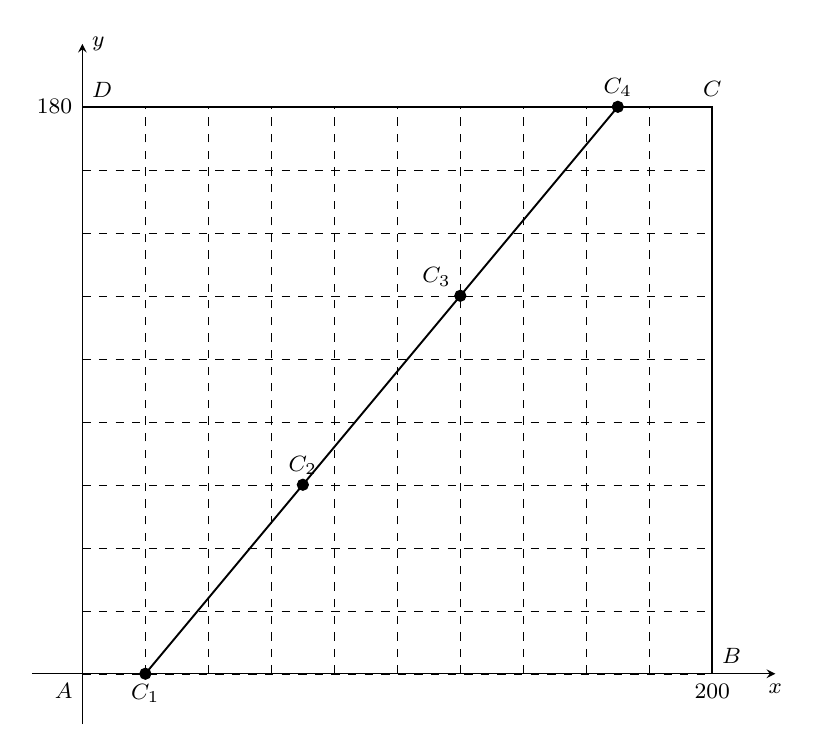
\begin{tikzpicture}[smooth,samples=300,scale=0.8,>=stealth,font=\footnotesize]
		\draw[->] (-0.8,0)--(11,0) node[below]{$x$};
		\draw[->] (0,-0.8)--(0,10) node[right]{$y$};
		\draw[line width=0.1pt,dashed] (0,0) grid (10,9);
		\draw (0,0) node[below left]{$A$};
		\draw[line width=0.7pt] (1,0)node[below]{$C_1$}--(8.5,9)node[above]{$C_4$};
		\draw[line width=0.7pt] (10,0)node[below]{$200$}--(10,9)node[above]{$C$}--(0,9)node[left]{$180$};
		\draw[fill=black] (1,0) circle(2.5pt) (3.5,3) circle(2.5pt) (6,6) circle(2.5pt) (8.5,9) circle(2.5pt);
		\node[above] at (3.5,3) {$C_2$};
		\node[above left] at (6,6) {$C_3$};
		\node[above right] at (10,0) {$B$};
		\node[above right] at (0,9) {$D$};
\end{tikzpicture}}
}
\end{vd}\dongcham{17}
\begin{dang}{Một số bài toán liên quan đến max - min}
	
\end{dang}


\begin{vd}%[0H1G4-3]%
	Trong mặt phẳng tọa độ $Oxy$, cho $A(-4;5)$, $B(-2;1)$. Tìm tọa độ của điểm $M$ trên trục tung sao cho $\left|\overrightarrow{MA}+\overrightarrow{MB}\right|$ ngắn nhất.
	\loigiai{
		Gọi $M(x;y) \in Oy \Rightarrow M(0;y)$.\\
		Ta có: $\heva{&\overrightarrow{MA}=(-4;5-y) \\& \overrightarrow{MB}=(-2;1-y)} \Rightarrow \overrightarrow{MA}+\overrightarrow{MB}=(-6;6-2y)$.\\
		$\Rightarrow \left|\overrightarrow{MA}+\overrightarrow{MB}\right|=\sqrt{72-24y+4y^2}=\sqrt{(2y-6)^2+36} \geq 6$.\\
		$\left|\overrightarrow{MA}+\overrightarrow{MB}\right|$ ngắn nhất là $6$. Dấu “=” xảy ra khi: $2y-6=0 \Leftrightarrow y=3$.\\
		Vậy $M(0;3)$.}
\end{vd}\dongcham{6}

\begin{vd}%[0H1G4-3]%
	Trong mặt phẳng tọa độ $ Oxy$, cho $ A(1;0)$, $ B(0;3)$, $ C(-3;-5)$. Tìm tọa độ điểm $ M$ thuộc trục $ Ox$ sao cho $\left|2\vec{MA}-3\vec{MB}+2\vec{MC}\right|$ nhỏ nhất.
	\loigiai{
		$M\in Ox\Rightarrow M(x;0)$.\\
		Ta có: $\vv{MA}=(1-x;0), \vv{MB}=(-x;3),\vv{MC}=(-3-x;-5)$.\\
		Suy ra: $2\vec{MA}-3\vec{MB}+2\vec{MC}=(-x-4;-19)$.\\
		Khi đó: $\left|2\vec{MA}-3\vec{MB}+2\vec{MC}\right|=\sqrt{(x+4)^2+19^2}\geq 19$.\\
		Do đó: $\left|2\vec{MA}-3\vec{MB}+2\vec{MC}\right|$ nhỏ nhất khi $x+4=0\Leftrightarrow x=-4$.\\
		Vậy $M(-4;0)$.
	}
\end{vd}\dongcham{6}

\boxmini{BÀI TẬP TỔNG HỢP TỰ LUYỆN}
\begin{baitap}%[BG Toán 10(2022)]%[Trần Hòa]%[0H1Y4-2]
	Trong mặt phẳng tọa độ $Oxy$, cho $\vec{u}=(1;2)$, $\vec{v}=(-3;4)$, $\vec{a}=(4;8)$
	\begin{enumerate}
		\item Hãy biểu  thị mỗi véc-tơ $\vec{u}$, $\vec{v}$, $\vec{a}$ theo các véc-tơ $\vec{i}$, $\vec{j}$.
		\item Tìm tọa độ $\vec{u}+\vec{v}$, $2\vec{u}$.
		\item Tìm mối liên hệ giữa véc-tơ $\vec{a}$ và $\vec{u}$.
	\end{enumerate}
	\loigiai{
		\begin{enumerate}
			\item Ta có $\vec{u}=\vec{i}+2\vec{j}$, $\vec{v}=-3\vec{i}+4\vec{j}$, $\vec{a}=6\vec{i}+8\vec{j}$.
			\item Ta có $\vec{u}+\vec{v}=(-2;6)$, $2\vec{u}=(2;4)$.
			\item Ta có $\vec{a}=4\vec{u}$.
		\end{enumerate}
	}
\end{baitap}\cham{8}
\begin{baitap}%[BG Toán 10(2022)]%[Trần Hòa]%[0H1Y4-2]
	Cho $\vec{u}=(2;-1)$, $\vec{v}=(4;5)$. Tính tọa độ các véc-tơ $\vec{u}+\vec{v}$, $\vec{u}-\vec{v}$, $3\vec{u}$, $5\vec{u}-4\vec{v}$.
	\loigiai{
		Ta có $\vec{u}+\vec{v}=(6;4)$, $\vec{u}-\vec{v}=(-2;-6)$, $3\vec{u}=(6;-3)$.\\
		Ta có $5\vec{u}=(10;-5)$, $4\vec{v}=(16;20)$ nên $5\vec{u}-4\vec{v}=(-6;-25)$.
	}
\end{baitap}\cham{12}

\begin{baitap}%[BG Toán 10(2022)]%[Trần Hòa]%[0H1B4-4]
	Cho $\vec{a}=(1;2)$, $\vec{b}=(3;-1)$. Hãy phân tích véc-tơ $\vec{c}=(-1;5)$ theo hai véc-tơ $\vec{a}$ và $\vec{b}$.
	\loigiai{
		Giả sử $\vec{c}=k\vec{a}+m\vec{b}=(k+3m;2k-m)$.\\
		Ta có $\heva{&k+3m=-1\\&2k-m=5}\Rightarrow \heva{&k=2\\&m=-1.}$\\ Vậy $\vec{c}=2\vec{a}-\vec{b}$.
	}
\end{baitap}\cham{8}

\begin{baitap}%[BG Toán 10(2022)]%[Trần Hòa]%[0H1B4-3]
	Cho tam giác $ABC$ có $A(-5;6)$, $B(-4;-1)$, $C(4;3)$.
	\begin{enumerate}
		\item Tìm tọa độ trung điểm $I$ của đoạn thẳng $AC$.
		\item Tìm tọa độ điểm $D$ sao cho tứ giác $ABCD$ là hình bình hành.
	\end{enumerate}
	\loigiai{
		\begin{enumerate}
			\item Gọi $I(x_I;y_I)$. Vì $I$ là trung điểm của của $AC$ nên
			\[\heva{&x_I=\dfrac{x_A+x_C}{2}=\dfrac{-5+4}{2}=-\dfrac{1}{2}\\&y_I=\dfrac{y_A+y_C}{2}=\dfrac{6+3}{2}=\dfrac{9}{2}.}\] Vậy $I\left(-\dfrac{1}{2};\dfrac{9}{2}\right)$.
			\item Gọi $D(x;y)$, ta có $\overrightarrow{AB}=(1;-7)$, $\overrightarrow{DC}=(4-x;3-y)$.
			\immini{$ABCD$ là hình bình hành khi $\overrightarrow{AB}=\overrightarrow{CD}\\\Leftrightarrow\heva{&1=4-x\\&-7=3-y}\Leftrightarrow\heva{&x=3\\&y=10} $. Vậy $D(3;10)$.}{\begin{tikzpicture}[scale=1,font=\footnotesize,line join = round, line cap = round, >= stealth]
					\coordinate (A) at (0,0);
					\def\a{3} \def\b{2}
					\coordinate (B) at ($(A)+(0:\a)$);
					\coordinate (D) at ($(A)+(70:\b)$);
					\coordinate (C) at ($(B)+(D)-(A)$);
					\draw (A)--(B)--(C)--(D)--cycle;
					\foreach \p/\g in {A/-90,B/-90,C/90,D/90} \draw[fill] (\p) circle(.5pt) node [shift={(\g:.3)}] {$\p$};
			\end{tikzpicture}}
		\end{enumerate}
	}
\end{baitap}\cham{12}

\begin{baitap}%[BG Toán 10(2022)]%[Trần Hòa]%[0H2B2-2]
	Cho $A(1;2)$, $B(-2;1)$, $C(2;-1)$.
	\begin{enumerate}
		\item Chứng minh tam giác $ABC$ vuông tại $A$.
		\item Tính diện tích tam giác $ABC$.
	\end{enumerate}
	\loigiai{
		\begin{enumerate}
			\item Ta có $\overrightarrow{AB}=(-3;1)$, $\overrightarrow{AC}=(1;-3)$, $\overrightarrow{BC}=(4;-2)$.\\
			Suy ra $AB=\sqrt{(-3)^2+1}=\sqrt{10}$, $AC=\sqrt{1^2+(-3)^2}=\sqrt{10}$, $BC=\sqrt{4^2+(-2)^2}=\sqrt{20}$.\\
			Ta thấy $AB^2+AC^2=10+10=20=BC^2$ nên tam giác $ABC$ vuông tại $A$.
			\item Vì tam giác $ABC$ vuông tại $A$ nên diện tích là $\dfrac{1}{2}AB\cdot AC=\dfrac{1}{2}\cdot \sqrt{10}\cdot \sqrt{10}=5$.
		\end{enumerate}
	}
\end{baitap}\cham{10}

\begin{baitap}%[0H1B4-5]
	Cho ba điểm $A(1;-1)$, $B(3;5)$, $C(2;2)$. 
	\begin{enumerate}
		\item Chứng minh rằng ba điểm $A$, $B$, $C$ thẳng hàng.
		\item Tìm tọa độ điểm $D$ trên $Ox$ sao cho $A$, $B$, $D$ thẳng hàng.
	\end{enumerate}
	\loigiai{
		\begin{enumerate}
			\item Ta có $\overrightarrow{AB}=(2;6)$, $\overrightarrow{AC}=(1;3)$.\\
			Vì $\dfrac{2}{1}=\dfrac{6}{3}$ nên $\overrightarrow{AB}$ và $\overrightarrow{AC}$ cùng phương do đó ba điểm $A$, $B$, $C$ thẳng hàng.
			\item Vì $D\in Ox$ nên $D(x;0)$. Ta có $\overrightarrow{AB}=(2;6)$, $\overrightarrow{AD}=(x-1;1)$.\\
			Ba điểm $A$, $B$, $D$ thẳng hàng khi $\dfrac{x-1}{2}=\dfrac{1}{6}\Rightarrow x-1=\dfrac{1}{3}\Rightarrow x=\dfrac{4}{3}$. Vậy $D\left(\dfrac{4}{3};0\right)$.
		\end{enumerate}
	}
\end{baitap}\cham{10}

\begin{baitap}%[0H1B4-3]
	Trong mặt phẳng $Oxy$ cho ba điểm $A(3; 4)$, $B(2; 1)$, $C(6; 3)$. Tìm tọa độ điểm $N$ thỏa mãn $2 \overrightarrow{NB}+ \overrightarrow{NC}- \overrightarrow{NA}= \overrightarrow{0}$.
	\loigiai{
		Giả sử $N(x;y)$.
		Ta có $\overrightarrow{NB}= (2-x; 1-y), \overrightarrow{NC}= (6-x; 3-y), \overrightarrow{NA}= (3-x; 4-y)$.\\
		Khi đó 
		\begin{align*}
			2 \overrightarrow{NB}+ \overrightarrow{NC}- \overrightarrow{NA}= \overrightarrow{0} &\Leftrightarrow \heva{&2(2-x)+(6-x)- (3-x)=0\\ &2(1-y)+ (3-y)- (4-y)=0}\\
			&\Leftrightarrow \heva{&7-2x=0\\ &1-2y=0} \Leftrightarrow \heva{&x= \dfrac{7}{2}\\ &y= \dfrac{1}{2}.}
		\end{align*}
		Vậy, $N \left(\dfrac{7}{2}; \dfrac{1}{2}\right)$ là điểm cần tìm.
	}
\end{baitap}\cham{10}

\begin{baitap}%[0H1B4-3]%[0H1K4-3]
	Trong mặt phẳng tọa độ $Oxy$, cho điểm $A(-3;5)$, $B(-4;-3)$, $C(1;1)$.
	\begin{enumerate}
		\item Tìm tọa độ điểm $D$ sao cho tứ giác $ABCD$ là hình bình hành.
		\item Tìm tọa độ điểm $K$ thuộc trục hoành sao cho $KA+KB$ nhỏ nhất.
	\end{enumerate}
	\loigiai{
		\begin{enumerate}
			\item Tứ giác $ABCD$ là hình bình hành \\
			$\Leftrightarrow\overrightarrow{AB}=\overrightarrow{DC}\Leftrightarrow (-1;-8)=(1-x_D;1-y_D)\Leftrightarrow\heva{&1-x_D=-1\\&1-y_D=-8}\Leftrightarrow\heva{&x_D=2\\&y_D=9.}$\\
			Vậy $D(2;9)$ là điểm cần tìm.
			\item Gọi $K(a;0)$ là điểm cần tìm.\\
			Ta có $KA+KB\ge AB$.\\
			Dấu \lq\lq$=$\rq\rq\, xảy ra khi $A,K,B$ thẳng hàng.\\
			$\Leftrightarrow \overrightarrow{AK}=k\overrightarrow{AB}\Leftrightarrow (a+3;-5)=k(-1;-8)\Leftrightarrow\heva{&a+3=-k\\&-5=-8k}\Leftrightarrow\heva{&a=-\dfrac{29}{8}\\&k=\dfrac{5}{8}.}$\\
			Vậy $K\left(-\dfrac{29}{8};0\right) $ thỏa yêu cầu bài toán.
		\end{enumerate}
	}
\end{baitap}\cham{15}

\begin{baitap}
	Trong mặt phẳng tọa độ $Oxy$, cho tam giác $ABC$ với $A(3;4)$, $B(4;1)$, $C(2;-3)$. Tìm tọa độ tâm $I$ của đường tròn ngoại tiếp tam giác $ABC$.
	\loigiai{
		\immini
		{Gọi $I(x;y)$ là tâm đường tròn ngoại tiếp tam giác $ABC$, khi đó ta có
			\begin{eqnarray*}
				& & \heva{&AI=BI\\ &AI=CI}\\
				& \Leftrightarrow & \heva{&\sqrt{(x-3)^2+(y-4)^2}=\sqrt{(x-4)^2+(y-1)^2}\\&\sqrt{(x-3)^2+(y-4)^2}=\sqrt{(x-2)^2+(y+3)^2}}\\
				& \Leftrightarrow & \heva{&2x-6y=-8\\ &2x+14y=12}\\
				& \Leftrightarrow & \heva{&x=-1\\ &y=1.}
			\end{eqnarray*}
			Vậy ta có $I(-1;1)$.}
		{\begin{tikzpicture}[line cap=round,line join=round,font=\footnotesize,>=stealth,scale=1]
				\fill ($(0,0)+(-125:2)$) coordinate [label=below left:$A$] (A) circle(1pt)
				($(0,0)+(5:2)$) coordinate [label=right:$B$] (B) circle(1pt)
				($(0,0)+(145:2)$) coordinate [label=above left:$C$] (C) circle(1pt)
				(0,0) coordinate [label=below:$I$] (I) circle(1pt);
				\draw (0,0) circle (2) 
				(A)--(B)--(C)--(A)--(I)--(B) (I)--(C);
		\end{tikzpicture}}
	}
\end{baitap}\cham{20}

